\item A particle of mass 100g is projected at time \( t = 0 \) with a speed 20 ms\(^{-1}\) at an angle \( 45^\circ \) to the horizontal as given in the figure. The magnitude of the angular momentum of the particle about the starting point at time \( t = 2s \) is found to be \( \sqrt{K} \) kg m\(^2\) / s. The value of \( K \) is \underline{\hspace{2.5cm}}. (Take \( g = 10 \) ms\(^{-2} \)).
    \begin{center}
        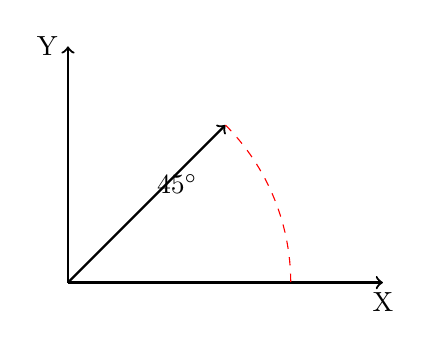
\begin{tikzpicture}
            \draw[thick, ->] (0,0) -- (4,0) node[anchor=north] {X};
            \draw[thick, ->] (0,0) -- (0,3) node[anchor=east] {Y};
            \draw[thick, ->] (0,0) -- (2,2) node[midway, above right] {\( 45^\circ \)};
            \draw[dashed, red] (2,2) arc[start angle=45, end angle=0, radius=2.83];
        \end{tikzpicture}
    \end{center}